\chapter{Architecture}\label{ch:met}

\section{Technologies used}
Firstly, the used technologies such as Spring, Mongo and Mallet will be briefly described in order
to easier follow project description later.
\subsection{Spring}
The Spring Framework is a comprehensive and widely used Java-based framework for building
enterprise-level applications. It provides a robust infrastructure for developing Java applications.
It simplifies the development of complex applications by promoting good design practices and
offering a suite of tools and libraries for building web applications, microservices, and
data-driven solutions. Additionally, Spring's modular architecture and extensive ecosystem
allow developers to use only the components they need, making it highly flexible and scalable.
\cite{spring}

\subsection{MongoDB}
MongoDB is a popular open-source, document-oriented NoSQL database designed for scalability,
flexibility, and performance. It stores data in flexible, JSON-like documents, allowing for varied
and dynamic data structures without requiring a fixed schema. MongoDB is known for its ability to handle large
volumes of data and its powerful querying and indexing capabilities. It supports a wide range of applications.
\cite{mongodb}

\subsection{Python}
Python is a versatile and high-level programming language known for its readability, simplicity, and extensive
standard library. It supports multiple programming paradigms, including procedural, object-oriented, and
functional programming. Python's dynamic typing and interpreted nature make it an excellent choice for rapid
application development. Python is also widely used in developing microservices due to its ease of use and
speed of development. \cite{python}

\subsection{Elasticsearch}
Elasticsearch is a powerful, open-source search and analytics engine designed for horizontal scalability,
reliability, and real-time search capabilities. It is built on Apache Lucene and provides a distributed, text
search engine with an HTTP web interface and schema-free JSON documents. It is commonly used for log and event
data analysis, full-text search, and real-time analytics due to its high performance, flexibility, and ability
to handle large volumes of data across distributed systems. \cite{elastic}

\subsection{Mallet}
MALLET (MAchine Learning for LanguagE Toolkit) is a Java-based open-source toolkit for statistical natural
language processing, particularly renowned for its implementations of topic modeling algorithms. It supports
various algorithms for discovering latent topics in large collections of text documents. MALLET provides tools
for preprocessing textual data, training topic models, and evaluating model performance. \cite{mallet}

\subsection{RabbitMQ}
RabbitMQ is a powerful open-source message broker that implements the Advanced Message Queuing Protocol (AMQP).
It enables seamless communication between distributed systems by acting as a mediator that facilitates the
reliable transfer of messages between applications and services. It supports various messaging patterns such
as point-to-point, publish/subscribe, and request/response. It is widely used in microservices architectures,
IoT applications, and asynchronous communication scenarios where decoupling and reliability are crucial.
\cite{rabbitmq}

\section{Design - overall architecture}
The project details are outlined below, supported by diagrams for better understanding.

\begin{figure}
    \centering
    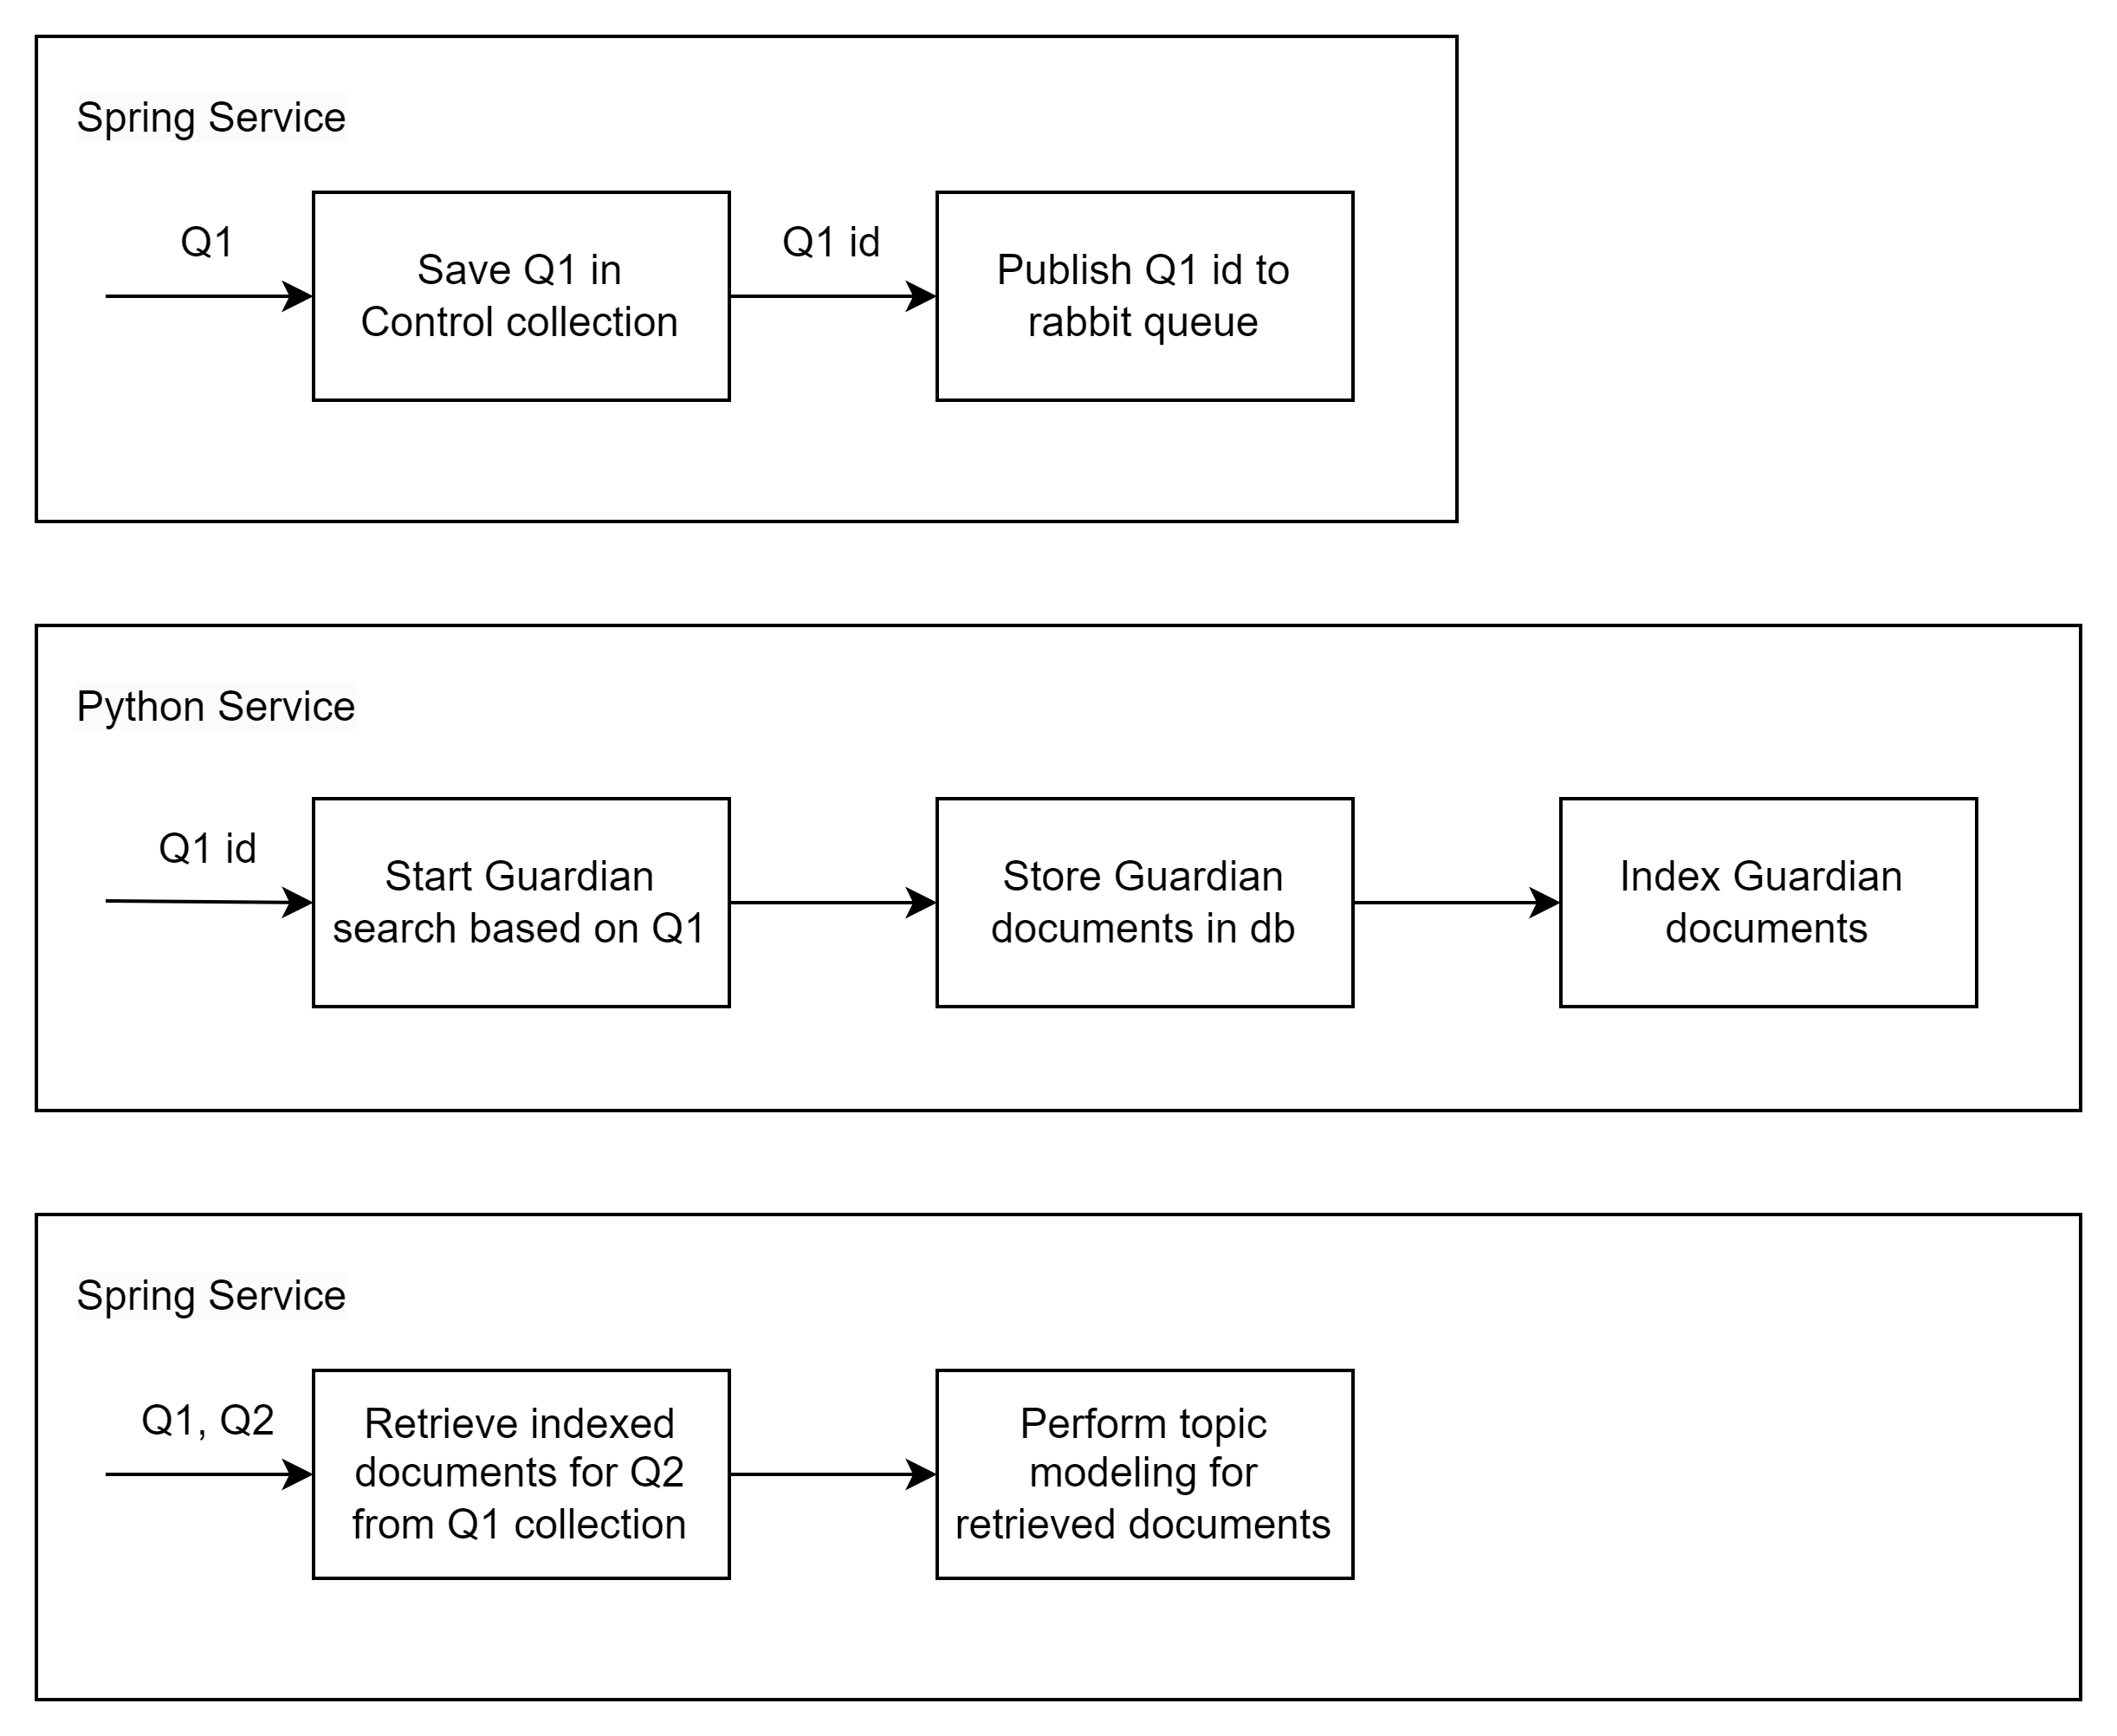
\includegraphics[width=0.7\linewidth] {././figures/diagram}
    \caption{Process flow}
\end{figure}

Firstly, the Spring service includes a monitoring functionality, initialized by a query referred to as Q1. An
example JSON representation of Q1 is shown in Listing \ref{lst:q1}.

\begin{lstlisting}[language=json, caption={JSON representation of Q1}, label={lst:q1}]
{
  "topic": "science",
  "local_start_date": "2024-05-01",
  "local_end_date": "2024-07-01"
}
\end{lstlisting}

This query is stored in a MongoDB collection named \textit{Control}, which manages all Q1 queries.
Listing\ref{lst:q1Class} shows class structure of Q1.

\begin{lstlisting}[language=Java, caption={Class definition of QOne}, label={lst:q1Class}]
String topic;

QOneStatus status;

LocalDateTime submitted_time;
LocalDateTime finished_time;

LocalDate local_start_date;
LocalDate local_end_date;
\end{lstlisting}

\textit{topic} field represents name of Q1, \textit{status} indicates the current processing status, which can
have the following values: SUBMITTED, PROCESSING and FINISHED. Beside that, \textit{local\_start\_date} and
\textit{local\_end\_date} are used to filter articles from Guardian API while \textit{submitted\_date} and
\textit{finished\_date} represent date of Q1 submission and date when the documents fetching for Q1 is finished,
respectively. Once saved in the database, the entity's ID is published to RabbitMQ.
\newline
Concurrently, a Python service subscribes to this queue. Upon receiving the Q1 ID, it triggers fetching from
the Guardian API, setting the Q1 document status to PROCESSING. Articles retrieved from the Guardian API are saved
in MongoDB in the format shown in Listing \ref{lst:article}.

\begin{lstlisting}[language=json, caption={JSON representation of a Guardian Article}, label={lst:article}]
{
    "title": title,
    "content" : content,
    "guardian_id" : guardian_id,
    "web_date": web_date
}
\end{lstlisting}

The \textit{title} and \textit{content} fields represent title and contect of an article respectively whereas
\textit{guardian\_id} and \textit{web\_date} represent guardian id and date of publishing an article. Each article
is subsequently indexed and stored as a JSON object in the Elasticsearch server.

For the second query, Q2, a user requests \textit{k} topics. This requires the Q1 ID as a parameter. For instance,
if Q1 was about \textit{Science}, and related articles are stored in the database, a subsequent Q2 query like
\textit{Nuclear war} expects to retrieve \textit{k} topics based on that subset of documents.

\section{Design for Spring service}

One of the services in our application is a Spring service, which is responsible for receiving all user requests,
saving Q1 in the database, pushing Q1's ID to RabbitMQ, retrieving documents from the ElasticSearch server, and
performing the topic modeling part. Figure \ref{fig:spring-structure} shows the structure of the Spring service.

\begin{figure}[ht]
  \centering
  \begin{forest}
    for tree={
      font=\ttfamily,
      grow=east,
      parent anchor=east,
      child anchor=west,
      edge path={
        \noexpand\path [draw, \forestoption{edge}] (!u.parent anchor) -- ++(5pt,0) |- (.child anchor)\forestoption{edge label};
      },
      l sep=15pt,
      s sep=15pt,
    }
    [awesomemodeling
      [controllers]
      [services]
      [repositories]
      [enums]
      [entities]
      [dtos]
      [AwesomemodelingApplication.java]
    ]
  \end{forest}
  \caption{Folder structure of the Spring service}
  \label{fig:spring-structure}
\end{figure}

During the development of the Spring service, we followed the \textit{Separation of Concerns} principle, which is a
fundamental principle in software engineering and design. It is used to separate an application into units with
minimal overlapping between the functions of the individual units \cite{geeksforgeeks:soc}. This is done by splitting
logic into three different layers: \textit{controllers}, \textit{services}, and \textit{repositories}.

The \textit{controllers} folder contains a class \textit{QOneController.java} responsible for handling HTTP requests
and mapping them to the appropriate service methods. This keeps the request handling logic separate from business
logic and data access logic.

The \textit{services} folder holds the business logic of the service—in our case, \textit{MalletService.java}. The
\textit{repositories} folder contains the data access logic, specifically an interface that extends
\textit{MongoRepository}—\textit{ControlRepository.java}. This separation allows us to change the data access layer
without affecting the business logic.

Another good design practice was creating \textit{entities} and \textit{dtos} folders. The \textit{entities} classes
represent the data models or domain objects. By keeping them in a separate folder, we ensure that the domain logic
is isolated from the rest of the application. The \textit{dtos} folder keeps \textit{Data Transfer Objects} classes
separately, which are used to transfer data between layers of the application, especially between the client and server.

\section{Design for Python service}
Another service that is part of our application is the Python service called \textit{downindex}, which is responsible for listening to incoming messages in \textit{RabbitMQ}, fetching articles from the \textit{Guardian API}, and indexing them using \textit{ElasticSearch}. The structure of this service is very simple and is shown in Figure \ref{fig:python-structure}. \textit{main.py} holds all the business logic of the service, while \textit{requirements.txt} lists all the required dependencies.

\begin{figure}[ht]
  \centering
  \begin{forest}
    for tree={
      font=\ttfamily,
      grow=east,
      parent anchor=east,
      child anchor=west,
      edge path={
        \noexpand\path [draw, \forestoption{edge}] (!u.parent anchor) -- ++(5pt,0) |- (.child anchor)\forestoption{edge label};
      },
      l sep=15pt,
      s sep=15pt,
    }
    [downindex
      [main.py]
      [requirements.txt]
    ]
  \end{forest}
  \caption{Folder structure of the Python service}
  \label{fig:python-structure}
\end{figure}


